% Working manuscript based on the author's draft supplied November 13, 2026.
% Required factual/documentation/notation corrections only; see REQUIRED_CHANGES.txt.
% Reporting-only amendment: HSA-week NSSP scoring is primary; saved predictions are unchanged.
\documentclass[conference,a4paper]{IEEEtran}
\usepackage[T1]{fontenc}
\usepackage[utf8]{inputenc}
\usepackage{amsmath,amssymb,graphicx,booktabs,array,tabularx,capt-of}
\usepackage[hyphens]{url}
\usepackage[hidelinks]{hyperref}
\graphicspath{{figures/}}
\raggedbottom
\newcolumntype{Y}{>{\raggedright\arraybackslash}X}
\title{Spatiotemporal Hybrid Ensemble Framework for Forecasting Respiratory Emergency Department Burden Using Syndromic Surveillance Data}
\author{\IEEEauthorblockN{Alexander Roque}
\IEEEauthorblockA{Department of Engineering\\Norfolk State University\\Norfolk, VA, USA\\a.d.roque@spartans.nsu.edu}
\and
\IEEEauthorblockN{Isaac Osunmakinde}
\IEEEauthorblockA{Department of Computer Science\\Norfolk State University\\Norfolk, VA, USA\\ioosunmakinde@nsu.edu}}
\begin{document}
\maketitle
\begin{abstract}
This study evaluates a retrospective one-week-ahead forecasting framework for respiratory surveillance that combines random forest, gradient boosting, and multilayer perceptron regressors. Target lags, rolling statistics, annual seasonal terms, and lagged auxiliary signals are augmented with K-means cluster indicators. Preprocessing and models are fitted within chronological boundaries, and ensemble weights are obtained from inverse validation mean squared error. Three independently retrained experiments use National Syndromic Surveillance Program (NSSP) emergency-department burden, contemporary ILINet outpatient influenza-like illness, and historical ILINet spanning the pandemic transition. Primary hybrid $R^2$ is 0.599, 0.890, and 0.895, respectively; root mean squared error is 0.972, 0.716, and 0.833 percentage points. NSSP scoring counts each health-service-area week once; the original reporting-record-weighted $R^2$ is 0.671. The hybrid improves root mean squared error over persistence and selected classical references in each experiment, although NSSP multilayer perceptron and contemporary ILINet gradient boosting are marginally better. Record-weighted checks show modest feature gains and competitive equal weighting. Final-test-window reuse limits confirmatory interpretation. The contribution is an auditable same-framework proof of concept, not fitted-model transfer or operational readiness.
\end{abstract}
\begin{IEEEkeywords}
respiratory forecasting, syndromic surveillance, ensemble learning, K-means, ARIMA, SARIMA
\end{IEEEkeywords}

\section{Introduction}
Weekly respiratory forecasts can support near-term healthcare planning, yet accuracy depends on the surveillance target, the epidemic regime, and the information available at each forecast origin. The Centers for Disease Control and Prevention (CDC) National Syndromic Surveillance Program (NSSP) quantifies respiratory emergency-department (ED) burden, while ILINet quantifies unweighted outpatient influenza-like illness (ILI) \cite{nssp,guide,ilinet}. These streams are related but non-interchangeable; a model fitted to one cannot be assumed to transfer to the other.

This study therefore asks whether a single, explicitly specified, availability-aligned forecasting procedure can be re-estimated across three settings under identical rules. The primary experiment evaluates the procedure on NSSP respiratory ED burden. An independently retrained contemporary ILINet experiment tests procedural portability. A historical ILINet experiment spanning the pandemic transition tests predictive performance under a major regime shift. Every experiment fits its own preprocessing, clusters, learners, ensemble weights, and classical benchmarks; no NSSP-trained model is transferred. The contribution is the coordinated evaluation of lagged surveillance inputs, K-means contextual indicators, heterogeneous regressors (random forest, gradient boosting, multilayer perceptron), inverse-validation-mean-squared-error (MSE) weighting, and same-row naive and classical time-series references. Descriptive geographic maps supply context without claiming spatial dependence. The completed-week availability assumption and reuse of final-test windows across all three experiments during auxiliary-lag development are stated explicitly: the results constitute an auditable retrospective proof of concept, not fitted-model transfer or operational readiness.

\section{Related Work}
\subsection{Time-Series Models and Ensemble Forecasting}
Real-time multi-model influenza ensembles (Reich et al.\ \cite{reich}) and the FluSight evaluations (Mathis et al.\ \cite{mathis}) demonstrate useful ensemble performance in their evaluated settings, rather than uniform superiority over individual models (Table~\ref{tab:prior}). Machine-learning studies of respiratory hospitalizations (Albrecht et al.\ \cite{albrecht}) and atypical respiratory syncytial virus (RSV) peaks (Morbey et al.\ \cite{morbey}) further demonstrate that nonlinear models must be judged against the specific outcome and epidemiological regime. Motivated by this literature, the present study uses a fixed, validation-derived convex combination of random forest, gradient boosting, and multilayer perceptron regressors as a design choice, not a literature-established preference over second-stage stacking. Same-row persistence, moving-average, seasonal-naive, autoregressive integrated moving-average (ARIMA), and seasonal ARIMA (SARIMA) references provide the comparison \cite{hyndman,box}.

\subsection{Integrated Surveillance and the Research Gap}
Multi-source influenza forecasting (Ray et al.\ \cite{ray}) demonstrates the value of integrating surveillance signals. Real-time syndromic algorithms (Evans and Sparks \cite{evans}) instead address timely outbreak detection from ED presentations (Table~\ref{tab:prior}). In the present forecasting task, auxiliary signals must respect the information boundary at each forecast origin. Contemporaneous pathogen shares, for example, cannot be treated as known when predicting the same week.

\textit{Research gap.} This study examines a bounded evaluation question: applying one fully specified, availability-aligned procedure---lagged surveillance inputs, clustering-derived context, heterogeneous regressors, chronological weighting, and identical same-row benchmarks---to heterogeneous national streams (NSSP respiratory ED burden and both contemporary and historical ILINet) under common evaluation rules, including a pandemic-transition stress test. It does not claim that ensembles, lag features, clustering, or classical baselines are themselves novel.

\begin{table}[t]
\par\noindent\begin{minipage}{\columnwidth}
\captionof{table}{Prior Machine Learning Studies in Healthcare Forecasting}
\label{tab:prior}\centering\footnotesize
\begin{tabularx}{\columnwidth}{@{}p{0.19\columnwidth}YY@{}}
\toprule
Study & Contribution relevant here & Evaluation boundary\\
\midrule
Reich \cite{reich} & Real-time influenza ensembles & Influenza-specific targets\\
Mathis \cite{mathis} & FluSight target and scoring design & Hospitalization outcome\\
Ray \cite{ray} & Multiple influenza data streams & Source availability matters\\
Morbey \cite{morbey} & ML epidemic-peak prediction & Atypical RSV season\\
Albrecht \cite{albrecht} & ML respiratory hospitalization forecasts & Different target and setting\\
Evans \cite{evans} & Real-time syndromic algorithms & Monitoring, not this burden target\\
\bottomrule
\end{tabularx}
\end{minipage}
\par\smallskip

\end{table}

\section{Methods}
\subsection{Data and Evaluation Windows}
Three independently partitioned experiments are analyzed. The primary experiment targets the combined respiratory ED-visit percentage reported by NSSP. Of 569,245 source rows, 245,165 contain a target and 230,918 contain the required target and lag features. These rows span 2,264 geographic keys: 2,215 county-indexed series carrying health-service-area (HSA) values and 49 state or national aggregate series. County labels can repeat the same HSA outcome. Primary NSSP scoring therefore counts each HSA-week once; the original mixed-source record-weighted scores remain a secondary comparison. This reporting choice was adopted after review, not prespecified. Training, validation weights, and predictions are unchanged.

Both ILINet experiments target the unweighted outpatient ILI percentage across 54 reporting groups. Contemporary ILINet contains 10,120 source rows and 9,550 modeled rows. Historical ILINet contains 14,199 source rows and 13,932 complete-case eligible rows, of which 11,070 enter the selected experiment (the remaining complete rows covering 2020-W40--2021-W39 are excluded). Table~\ref{tab:data} reports the exact chronological partitions used for fitting, validation, and final testing in each experiment.

Missing targets or required lagged predictors cause complete-case exclusion. No median imputation or raw geographic-category encoding is applied. All three experiments are re-estimated independently; no model fitted on one stream is transferred to another.

\begin{table*}[t]
\par\noindent\begin{minipage}{\textwidth}
\captionof{table}{Chronological Partitions; Complete Epidemiological Weeks Stay Together}
\label{tab:data}\centering\footnotesize
\begin{tabularx}{\textwidth}{@{}lYYY@{}}
\toprule
Experiment & Pre-test history & Fit / validation rows (weeks) & Final-test interval and rows\\
\midrule
1: NSSP & Oct. 22, 2022--May 4, 2024; 183,384 rows & 144,896 (64) / 38,488 (17); validation starts 2024-W02 & May 11--Sep. 28, 2024; 47,534 prediction records; 13,356 primary HSA-weeks (21 weeks)\\
2: Contemporary ILINet & 2022-W43--2025-W30; 7,776 rows & 6,210 (115) / 1,566 (29); validation starts 2025-W02 & 2025-W31--2026-W14; 1,774 rows (37 weeks)\\
3: Historical ILINet & 2016-W43--2019-W39; 8,262 rows & 6,588 (122) / 1,674 (31); validation starts 2019-W09 & 2019-W40--2020-W39; 2,808 rows (52 weeks)\\
\bottomrule
\end{tabularx}
\end{minipage}
\par\smallskip

\end{table*}

\subsection{System Design and Forecast Inputs}
Fig.~\ref{fig:system} and Algorithm~1 summarize the two-phase design applied independently to each experiment. Earlier pre-test weeks fit the scaler, K-means centroids, and supervised learners. The latest 20\% of pre-test weeks estimate inverse-MSE ensemble weights and select classical orders. With those choices fixed, all objects are rebuilt on the complete pre-test history. Final evaluation is rolling one-week-ahead: completed observations become inputs for the subsequent forecast, but parameters are not fitted to final-test outcomes within each run.

\begin{figure}[t]
\par\noindent\begin{minipage}{\columnwidth}
\centering
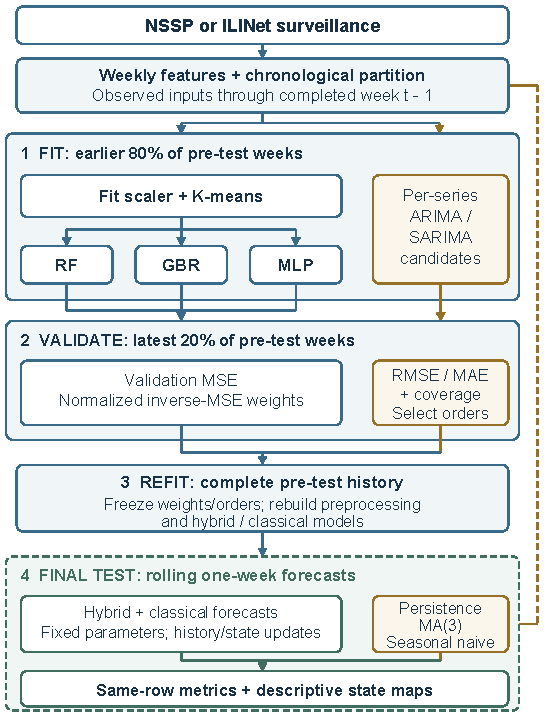
\includegraphics[width=\columnwidth]{framework_vector.pdf}
\captionof{figure}{System design, fitted independently for each experiment. Blue stages separate fitting, validation, and full-pretest refitting; amber branches show benchmarks. Final testing uses completed-week inputs without parameter refitting. Historical test reuse during development remains a separate limitation.}
\label{fig:system}
\end{minipage}
\par\smallskip

\end{figure}

For target $y_{r,t}$ at reporting unit $r$ and week $t$, inputs use observations through $t-1$. Features comprise target lags 1--3; the preceding three-week mean and sample standard deviation (denominator 2); and the annual phase terms $\sin(2\pi w_t/52)$ and $\cos(2\pi w_t/52)$. NSSP additionally receives the one-week-lagged COVID-19, influenza, and RSV visit shares; ILINet receives the one-week-lagged provider count. Current-week shares, smoothed values, and trend inputs are excluded. Completed-week data are assumed immediately available. Under the implemented denominator, Week 53 receives the same seasonal phase as Week 1; the seasonal-naive reference uses a 52-observation shift. Source epidemiological weeks include CDC 2025-W53 \cite{week53}.

Each experiment fits its own scaler, clusters, learners, weights, and classical models. Reuse of the three final-test windows during auxiliary-lag development remains a disclosed limitation.

\subsection{Clustering and Supervised Ensemble}
Features are standardized with means and standard deviations estimated on the current fitting segment $\mathcal F$ only. K-means \cite{macqueen} minimizes within-cluster squared Euclidean distance:
\begin{equation}
\min_{\{\mu_k\},\{c_i\}}\sum_{i\in\mathcal F}\|\mathbf z_i-\mu_{c_i}\|^2,
\qquad \tilde{\mathbf x}_i=[\mathbf z_i,\mathbf h(c_i)],
\label{eq:k}
\end{equation}
where $\mathbf z_i$ is the standardized feature vector and $\mathbf h(c_i)$ is a one-hot cluster indicator. Fit-only NSSP diagnostics selected $K=4$ as the largest elbow distance (silhouette 0.308); $K=2$ yielded a higher silhouette (0.484) but coarser separation. Thus $K=4$ is an elbow-supported parsimonious choice, not the silhouette optimum. The same $K$ is retained across experiments with newly estimated centroids (seed 42, 10 initializations). Full-pretest silhouettes of approximately 0.26--0.30 indicate overlapping regimes.

The learners supply complementary structures: random forest (RF; 150 trees, unlimited depth), gradient boosting regressor (GBR; 150 estimators, maximum depth 3, learning rate 0.05), and multilayer perceptron (MLP; hidden layers (32,16), ReLU, Adam, at most 300 iterations). The MLP internal early-stopping subset is a random 15\% of the rows supplied to each fit, not a chronological split. Validation observations $\mathcal V$ determine inverse-MSE weights:
\begin{equation}
E_j=\frac{1}{|\mathcal V|}\sum_{i\in\mathcal V}(y_i-\hat y_{j,i})^2,
\end{equation}
\begin{equation}
w_j=\frac{1/\max(E_j,10^{-12})}{\sum_l1/\max(E_l,10^{-12})},
\label{eq:weights}
\end{equation}
\begin{equation}
\hat y_i=\sum_jw_jf_j(\tilde{\mathbf x}_i),\qquad \sum_jw_j=1.
\label{eq:hybrid}
\end{equation}
Weights are frozen after validation and remain fixed during full-pretest refitting and final testing. The procedure is a transparent convex combination, not second-stage stacking; archived record-weighted checks also find equal weighting competitive. Full settings, cluster diagnostics, and profiles appear in Supplement S1; experiment-specific weights appear in S3.

\begin{table}[t]
\par\noindent\begin{minipage}{\columnwidth}
\centering\textbf{Algorithm 1: Proposed Hybrid Spatiotemporal Forecasting Framework}\par\smallskip
\centering\footnotesize
\begin{tabularx}{\columnwidth}{@{}lX@{}}
\toprule
\multicolumn{2}{l}{\textbf{Inputs}}\\
I. & NSSP and contemporary/historical ILINet surveillance panels.\\
II. & Target and auxiliary history available through the completed week.\\
\midrule
\multicolumn{2}{l}{\textbf{Procedure}}\\
III. & Load data; harmonize types and source-week identifiers.\\
IV. & Order each series; identify missing or invalid source values.\\
V. & Define whole-week fit, validation, and final-test boundaries.\\
VI. & Build target lags, rolling summaries, annual phase, and lag-1 auxiliary inputs. Exclude rows missing target/required features; apply week partitions; fit scaling on the fit segment.\\
VII. & Fit K-means on that segment; derive and append one-hot cluster indicators.\\
VIII. & Fit RF, GBR, and MLP; predict the later validation segment.\\
IX. & Select classical orders by validation; compute weights with (\ref{eq:weights}); freeze both. Refit the scaler, K-means, learners, and classical models on all pre-test rows; combine learner forecasts with (\ref{eq:hybrid}).\\
X. & Score all methods on matched units: HSA-weeks for primary NSSP, reporting rows for ILINet. Retain NSSP record-weighted comparisons.\\
XI. & Summarize temporal errors and descriptive state maps.\\
XII. & Repeat independently for each surveillance experiment.\\
\midrule
\multicolumn{2}{l}{\textbf{Outputs}}\\
XIII. & One-week forecasts, metrics, ablations/sensitivities, and test-period geographic summaries.\\
\bottomrule
\end{tabularx}
\end{minipage}
\par\smallskip

\end{table}

\begin{table*}[!t]
\par\noindent\begin{minipage}{\textwidth}
\captionof{table}{Same-Unit Final-Test Performance; Bold Indicates the Smallest MAE/RMSE or Largest $R^2$ Within Each Experiment}
\label{tab:results}\centering\footnotesize
\begin{tabular}{@{}lrrrrrrrrr@{}}
\toprule
&\multicolumn{3}{c}{NSSP HSA-weeks ($n=13,356$)}&\multicolumn{3}{c}{Contemporary ILINet ($n=1,774$)}&\multicolumn{3}{c}{Historical ILINet ($n=2,808$)}\\
\cmidrule(lr){2-4}\cmidrule(lr){5-7}\cmidrule(l){8-10}
Model & MAE & RMSE & $R^2$ & MAE & RMSE & $R^2$ & MAE & RMSE & $R^2$\\
\midrule
Hybrid &\textbf{0.6182}&0.9725&0.5986&\textbf{0.399}&0.716&0.890&\textbf{0.466}&\textbf{0.833}&\textbf{0.895}\\
RF &0.6497&1.0225&0.5562&0.412&0.728&0.886&0.481&0.854&0.889\\
GBR &0.6495&1.0337&0.5465&0.407&\textbf{0.715}&\textbf{0.891}&0.473&0.850&0.890\\
MLP &0.6186&\textbf{0.9723}&\textbf{0.5987}&0.416&0.766&0.874&0.476&0.849&0.891\\
ARIMA &0.7330&1.1231&0.4647&0.469&0.838&0.850&0.504&0.899&0.877\\
Annual SARIMA &0.8307&1.2882&0.2957&0.424&0.739&0.883&0.490&0.851&0.890\\
Persistence &0.6318&1.0914&0.4945&0.507&0.908&0.823&0.522&0.922&0.871\\
Moving average (3) &0.7032&1.1149&0.4724&0.721&1.286&0.646&0.714&1.194&0.784\\
Seasonal naive &0.9667&1.5395&-0.0059&1.029&1.686&0.391&1.033&1.648&0.588\\
\bottomrule
\end{tabular}
\par\smallskip\raggedright\footnotesize
\textit{Note:} MAE and RMSE are in percentage points; $R^2$ is dimensionless. Bold identifies the best observed score, not statistical significance.
\end{minipage}
\par\smallskip

\end{table*}

\subsection{Baselines and Evaluation}
Naive forecasts are the previous observation $y_{r,t-1}$, the preceding three-week mean, and the seasonal lag $y_{r,t-52}$. The ARIMA grid is limited to orders (1,0,0), (0,1,1), and (1,1,0). Annual SARIMA combines a nonseasonal order from $\{(1,0,0),(2,0,0),(1,0,1)\}$ with seasonal order $(1,0,0)_{52}$. Within each family and experiment, pooled validation root mean squared error (RMSE), then mean absolute error (MAE), selects an order subject to a 95\% coverage requirement. Selected orders are refitted with limited-memory Broyden--Fletcher--Goldfarb--Shanno (L-BFGS) optimization on complete pre-test history; during testing the state is updated without parameter refitting.

Metrics use identical eligible units for all methods: MAE and RMSE in percentage points, $R^2$, and supplementary symmetric mean absolute percentage error (SMAPE), bias, and correlation. Primary NSSP scoring restricts saved predictions to HSA-source records and averages targets and forecasts within HSA-week, yielding 636 HSAs over 21 weeks. ILINet retains reporting-unit-week scoring. Comparisons remain within experiments. All three final-test windows were inspected during auxiliary-lag development; results are exploratory, not untouched confirmatory tests. Supplement S1 archives classical search diagnostics, S2 development history, and S4 both NSSP scoring bases.

\begin{figure*}[!t]
\par\noindent\begin{minipage}{\textwidth}
\centering
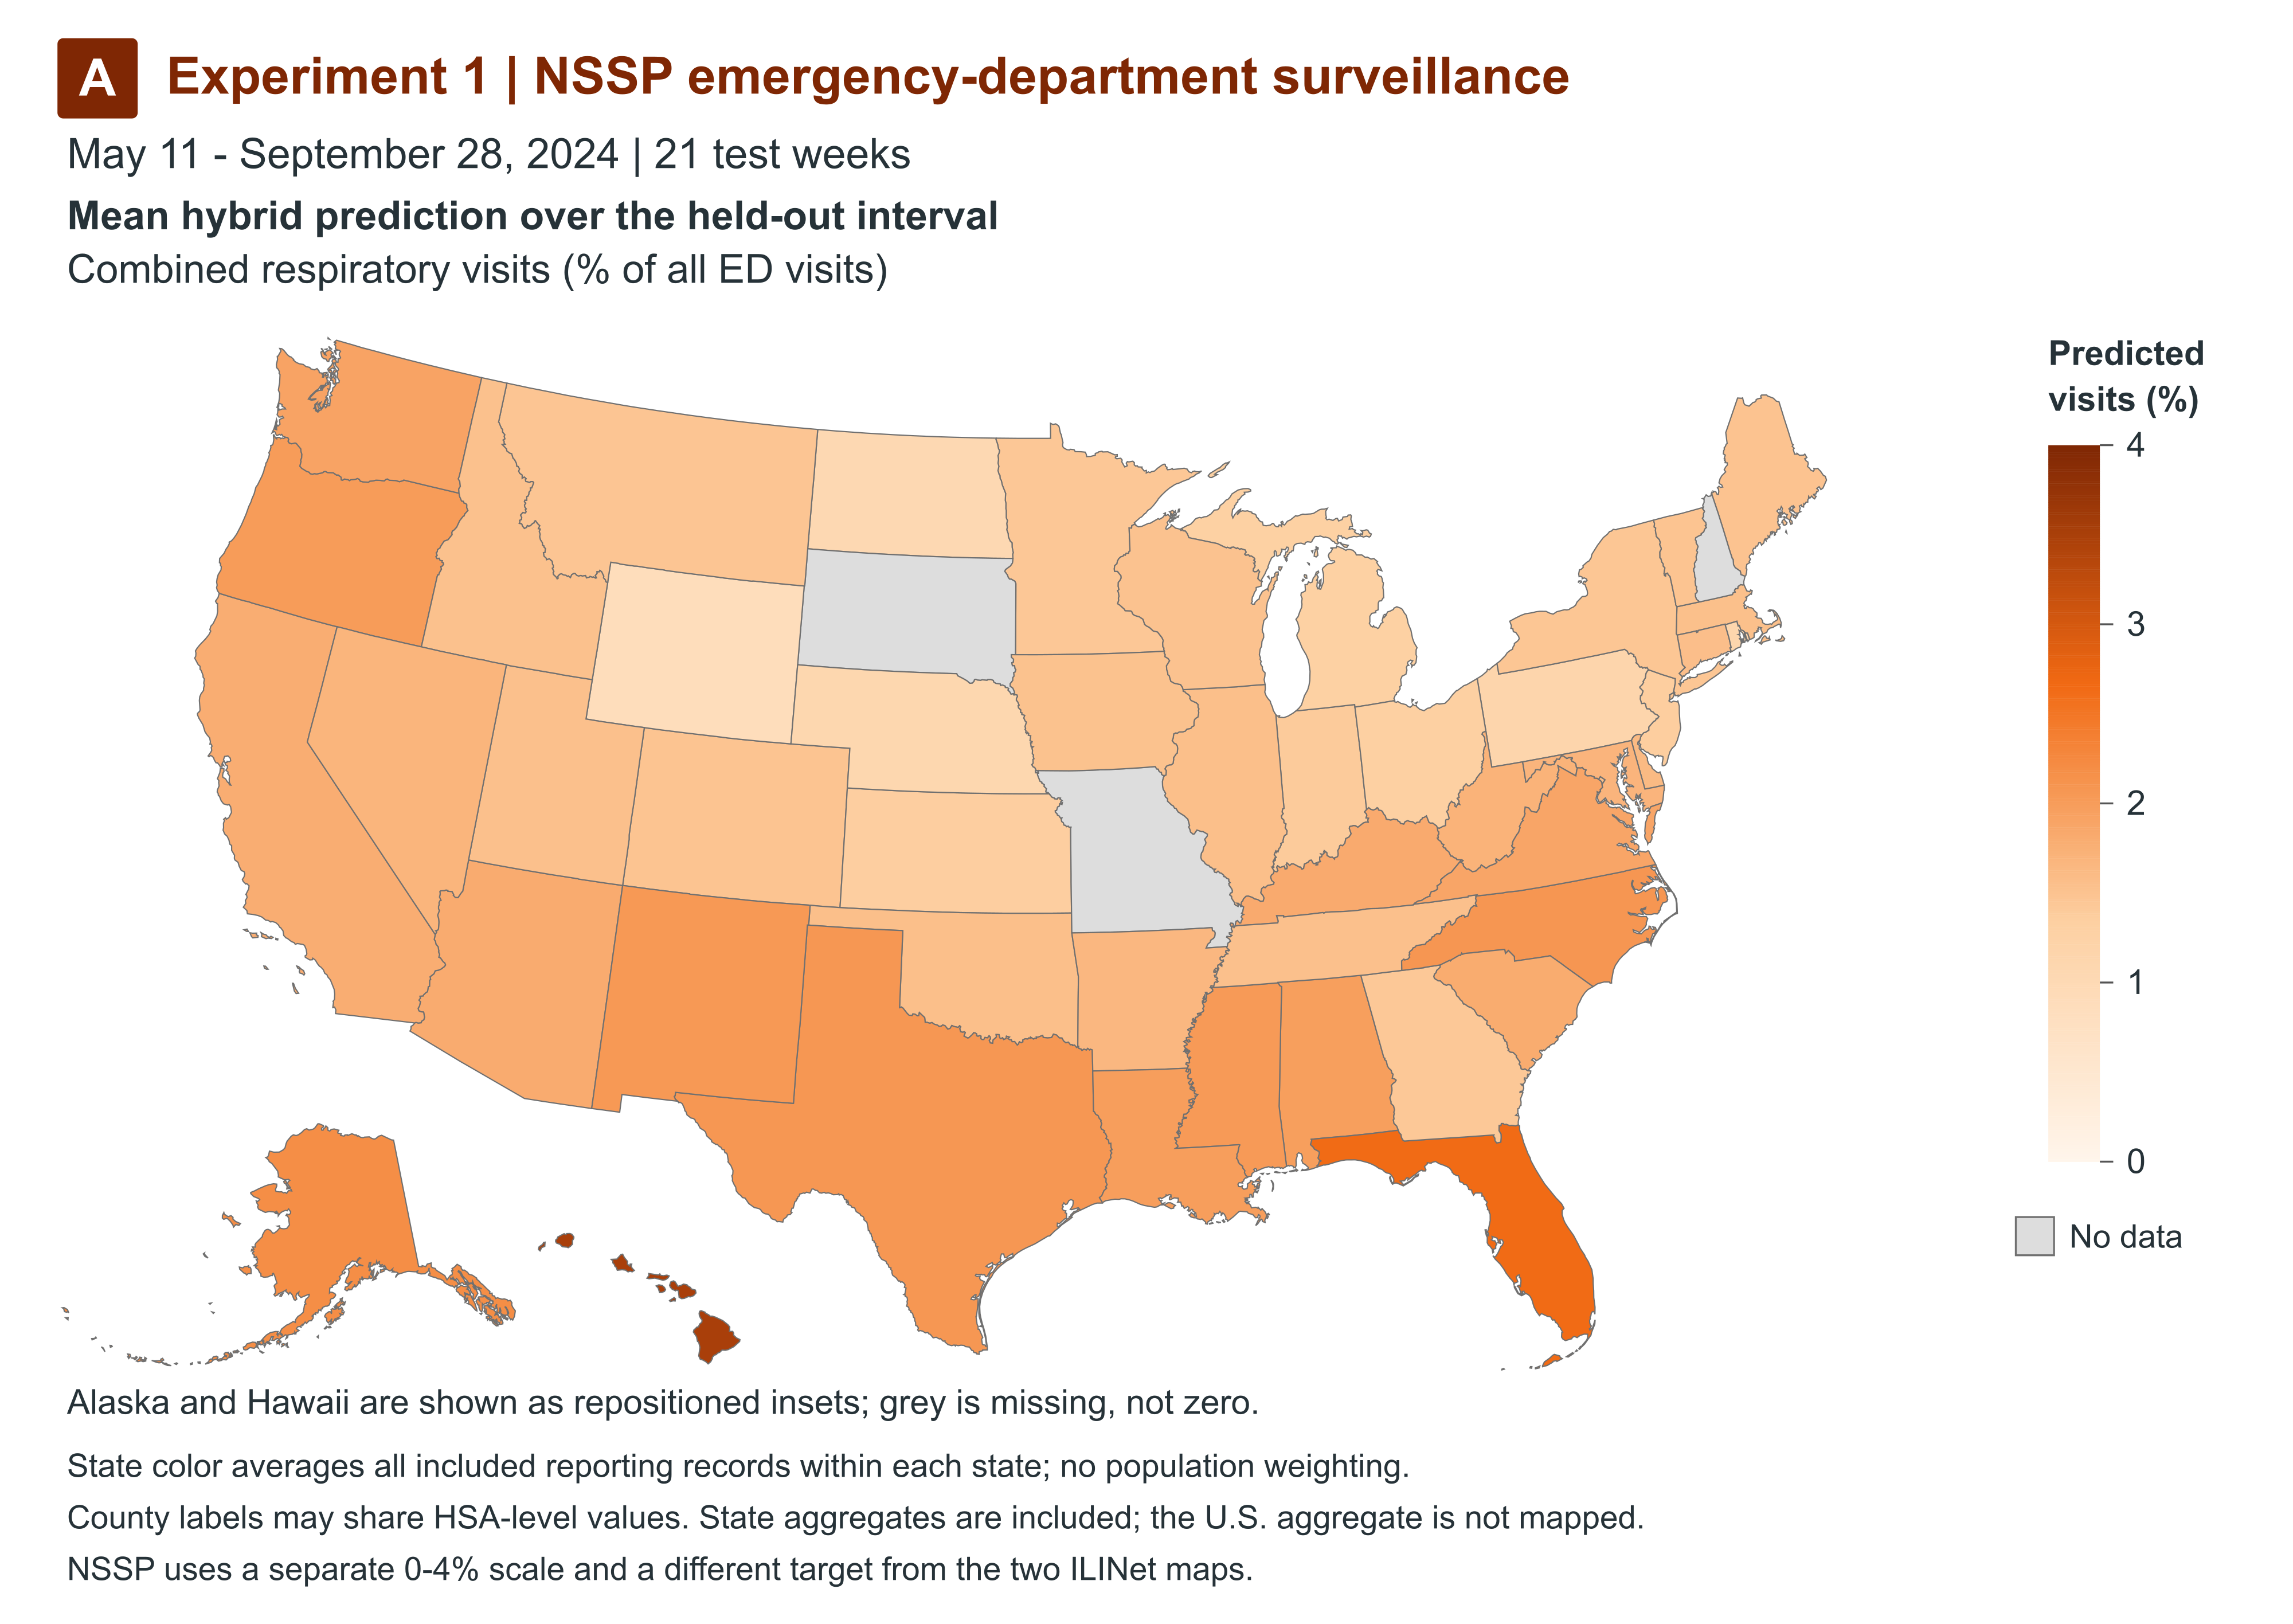
\includegraphics[width=0.48\textwidth]{fig13.png}\hfill
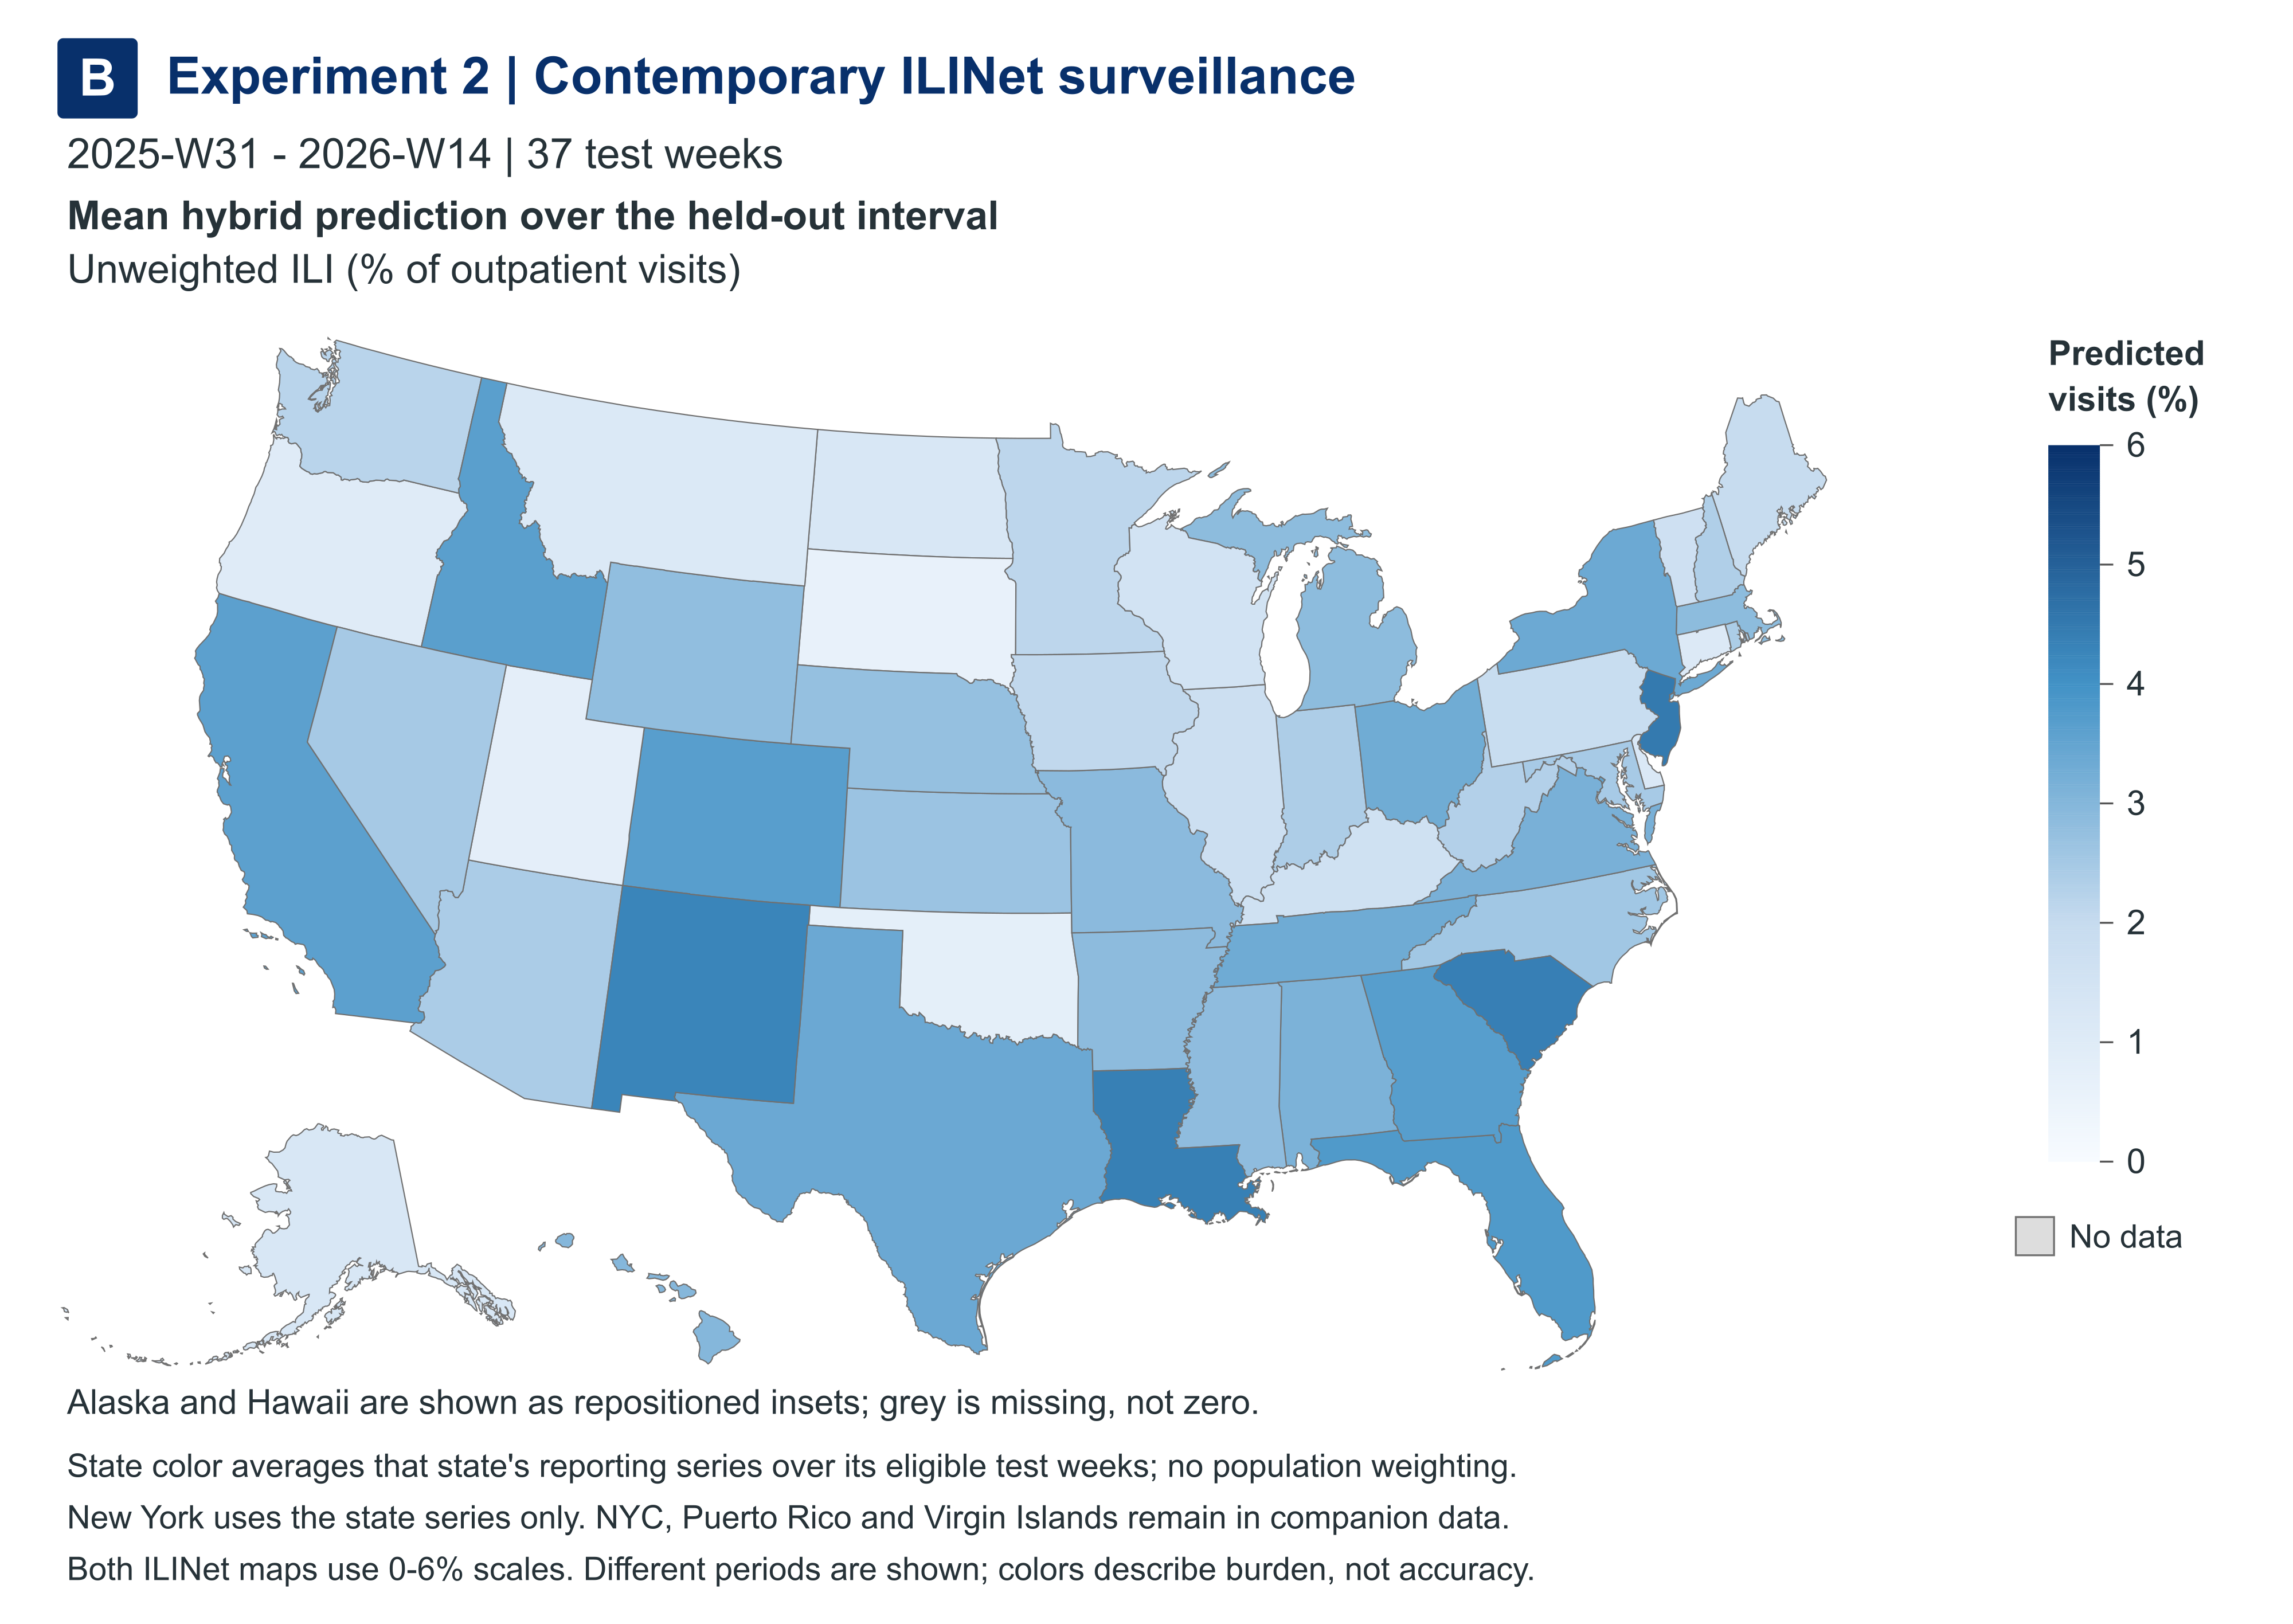
\includegraphics[width=0.48\textwidth]{fig14.png}\\[3pt]
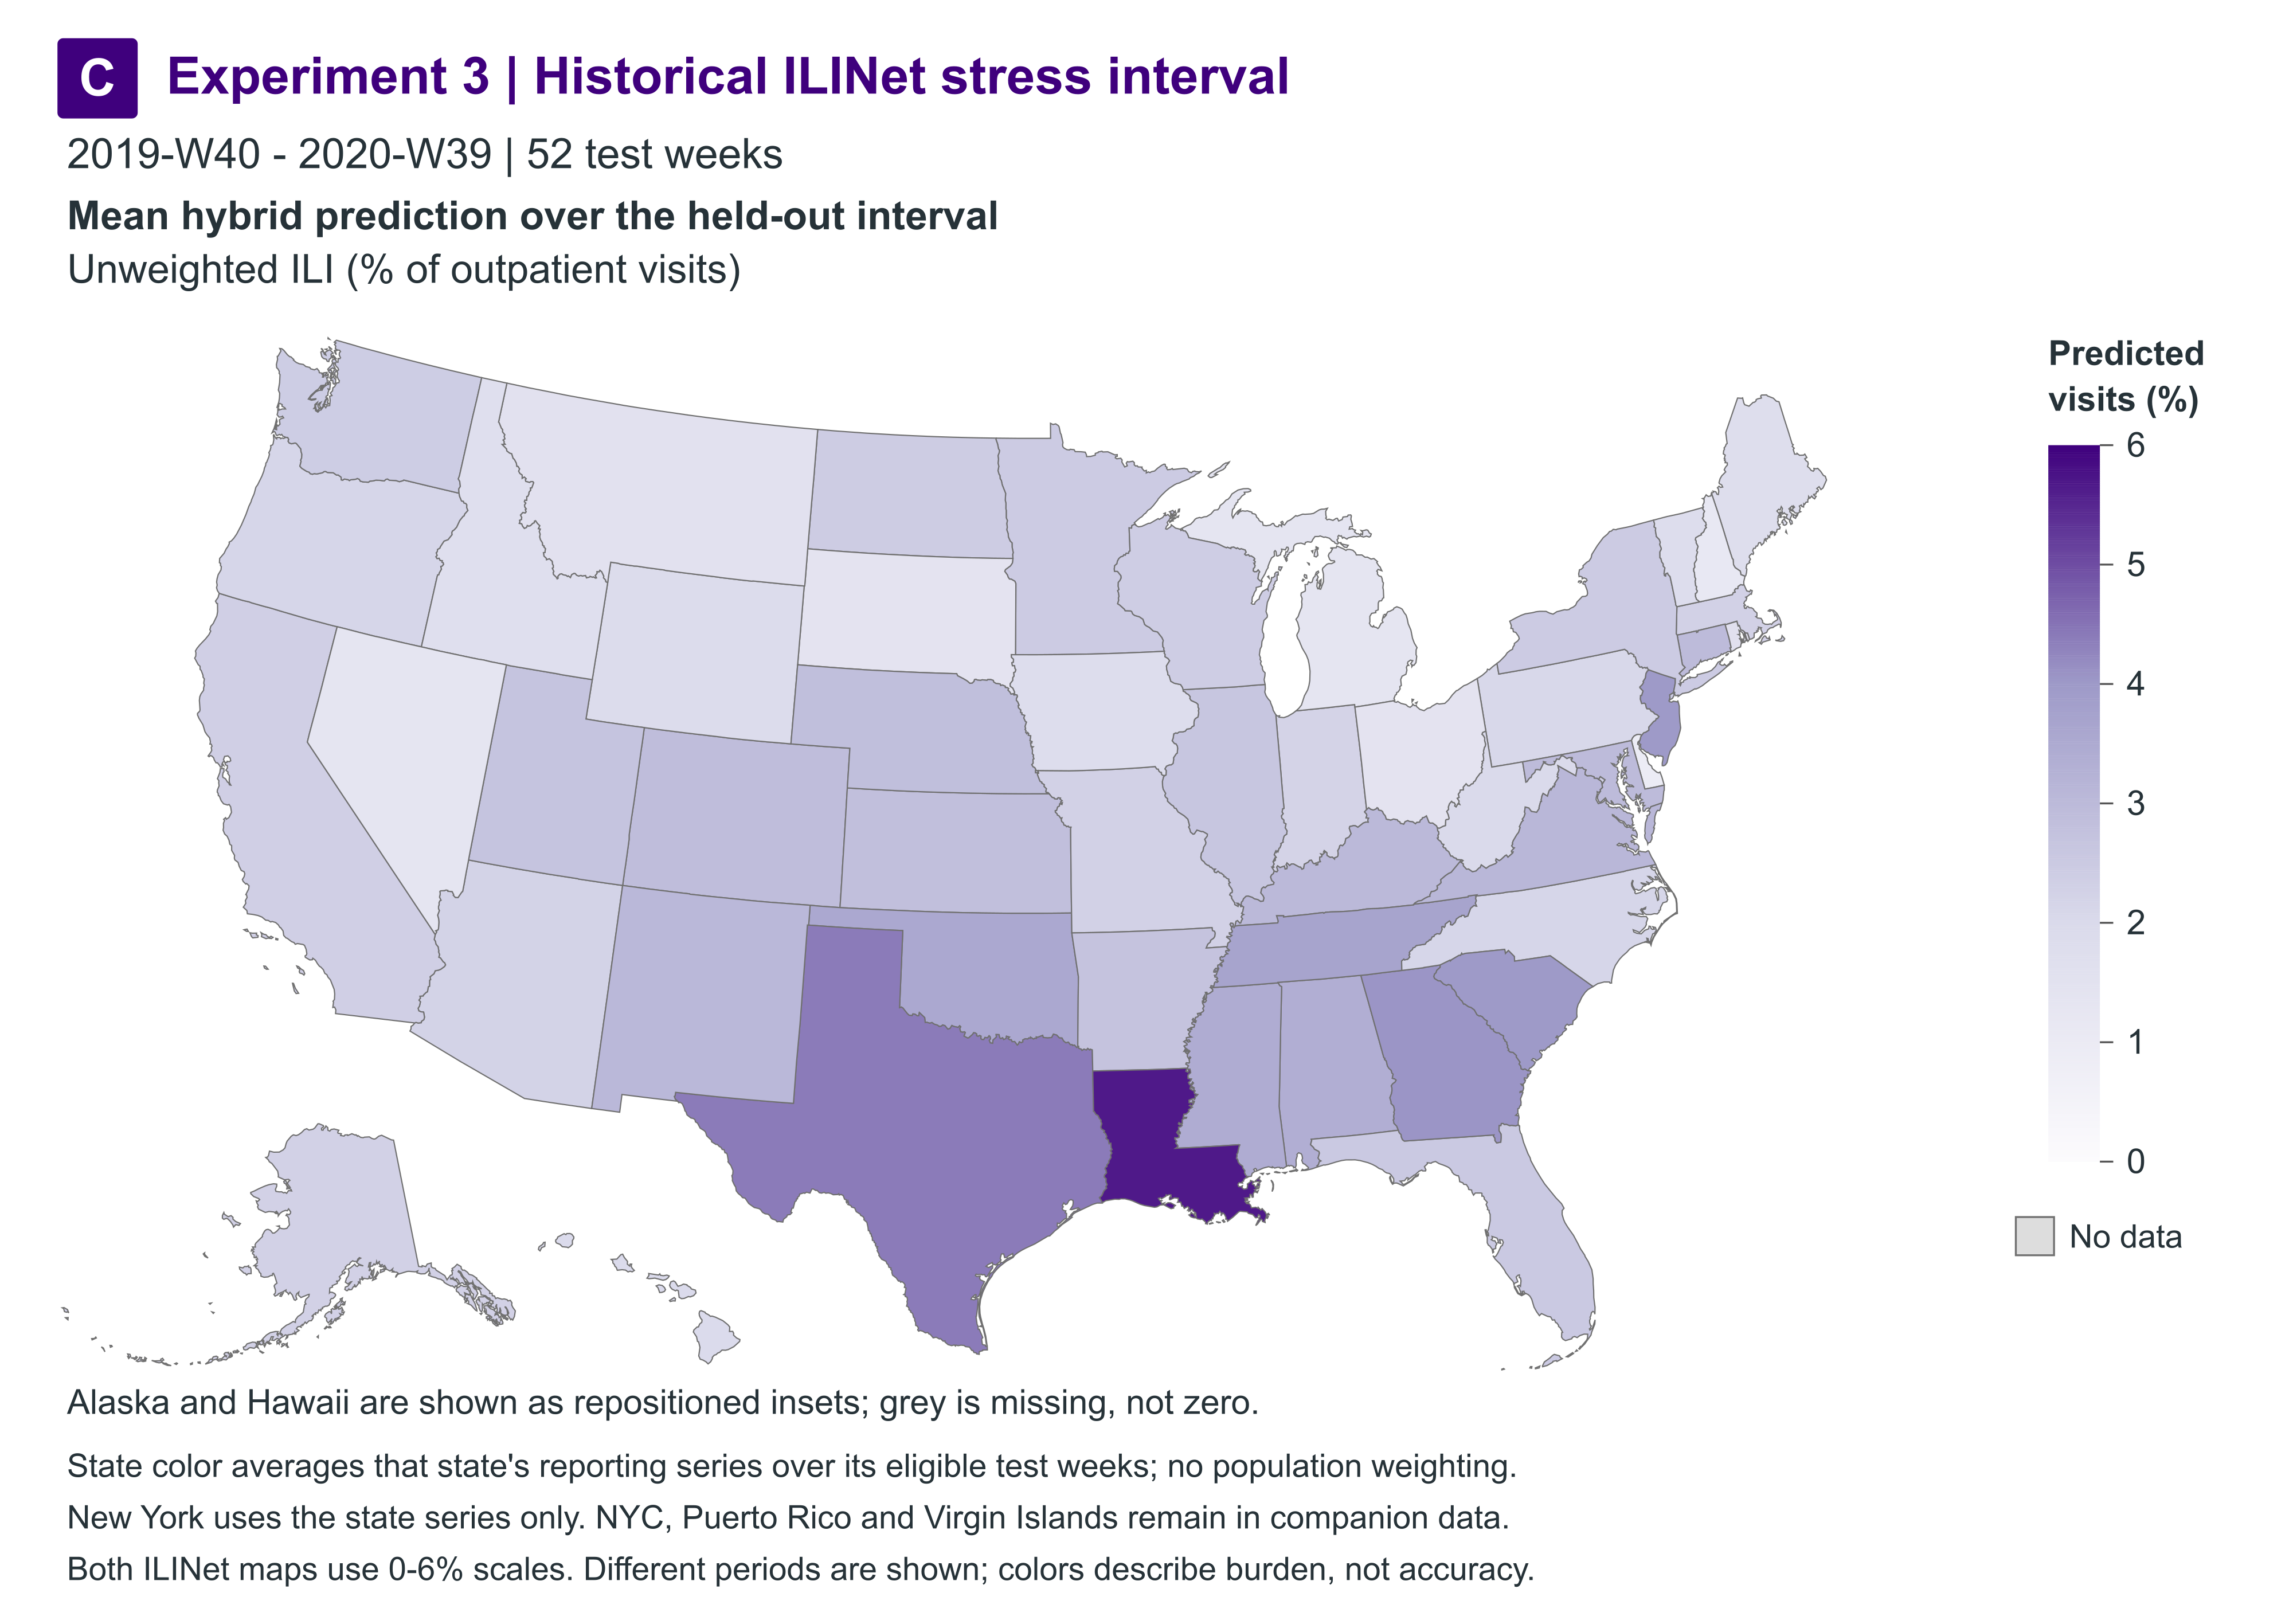
\includegraphics[width=0.48\textwidth]{fig15.png}
\captionof{figure}{Heat maps of mean held-out hybrid predictions: (A) NSSP respiratory ED visits; (B) contemporary ILINet unweighted ILI; (C) historical ILINet unweighted ILI. Targets and test periods differ. ILINet panels share a numerical scale; NSSP has its own scale. Darker colors indicate higher predicted percentages; gray indicates missing eligible data. Alaska and Hawaii are insets. Supplement S6 retains full-size maps; the map-values CSV supplies exact values, row counts, observed means, and bias.}
\label{fig:maps}
\end{minipage}
\par\smallskip

\end{figure*}

\section{Results}

\subsection{NSSP Forecasting}
On 13,356 HSA-weeks, the hybrid achieved primary NSSP RMSE 0.972 and $R^2=0.599$ (Table~\ref{tab:results}). RMSE was 10.9\% lower than persistence and 13.4\%/24.5\% lower than the selected ARIMA/SARIMA references. The hybrid had the lowest MAE, but MLP was marginally better on RMSE (0.972310 versus 0.972459) and $R^2$. Persistence retained a lower SMAPE. The original mixed-source comparison scores 47,534 records and yields hybrid RMSE 0.803 and $R^2=0.671$. Restriction to HSA-source records alone yields $R^2=0.669$; counting repeated HSA-weeks once accounts for most of the remaining difference. Targets and hybrid predictions agree within every HSA-week, so the change reflects weighting, not new forecasts.

\subsection{Contemporary and Historical ILINet}
Independent retraining on contemporary ILINet (1,774 rows) produced hybrid RMSE 0.716 and $R^2=0.890$, improving on persistence by 21.1\% and on the selected ARIMA/SARIMA references by 14.5\%/3.2\%. Gradient boosting was marginally superior on RMSE (0.715). On the historical ILINet pandemic-transition window (2,808 rows), the hybrid reached RMSE 0.833 and $R^2=0.895$, improving on persistence by 9.6\% and on ARIMA/SARIMA by 7.3\%/2.1\%, and achieving the lowest MAE and RMSE among the compared methods. In both ILINet experiments the hybrid's weekly-mean peak lagged the observed peak by one surveillance week (contemporary: 2025-W53 versus 2025-W52; historical: 2020-W01 versus 2019-W52). These delayed peaks qualify claims of turning-point accuracy despite favorable pooled scores. Neither experiment supports causal inference about pandemic policy or pathogen emergence. Supplement S7 retains the temporal trajectories.

\subsection{Sensitivity Findings}
Archived record-weighted NSSP ablations raised RMSE from 0.803 to 0.823 without clustering and to 0.806 without pathogen-component lags ($R^2=0.655$ and 0.669). These modest conditional effects were not evaluated on the primary HSA-week basis. Equal-weight rescoring yielded RMSE 0.801147, 0.716932, and 0.833380 across the three experiments, versus inverse-MSE values 0.803473, 0.716087, and 0.833458; NSSP again uses the original record weighting. Inverse-MSE weighting is not uniformly superior under these comparisons. Separate target-lag, rolling-summary, and seasonal-term ablations and seasonal weight-stability tests remain unperformed. Supplements S2--S4 retain the numerical details and scoring definitions.

\subsection{Geographic Interpretation}
Fig.~\ref{fig:maps} displays unchanged mean held-out hybrid predictions. NSSP (orange scale, 0--4\%) averages reporting records, including repeated HSA assignments and available state aggregates. These descriptive maps retain record weighting, unlike primary HSA-week scoring; their values are neither official state rates nor population-weighted estimates. Contemporary and historical ILINet (shared range, 0--6\%, with distinct blue and purple palettes) use state series, with New York City, Puerto Rico, and the Virgin Islands separate in companion data. Gray indicates missing eligible data, not zero. The maps do not identify validated hotspots, spatial autocorrelation, or density associations; those earlier claims have been withdrawn.

\subsection{Architectural Comparison}
Table~\ref{tab:architecture} distinguishes the roles of the surveillance streams, the naive and classical baselines, and the proposed framework. National streams supply the weekly observations; the baselines isolate recent-level or seasonal predictability without auxiliary signals or spatial models; the framework combines lagged inputs, rolling and seasonal terms, lagged auxiliary signals, and K-means context with heterogeneous learners, evaluated under one chronological procedure across three independently refitted experiments. The comparison is structural, not a cross-study accuracy ranking.

\begin{table}[!ht]
\par\noindent\begin{minipage}{\columnwidth}
\captionof{table}{Architectural Comparison of Referenced Streams and Methods}
\label{tab:architecture}\centering\footnotesize
\begin{tabularx}{\columnwidth}{@{}p{0.23\columnwidth}YY@{}}
\toprule
Reference & Role / temporal inputs & Learning and geographic output\\
\midrule
NSSP / ILINet & National surveillance streams; weekly observations & Data sources, not forecasting architectures\\
Naive references & Last value, local mean, annual lag & No fitted learner or spatial model\\
ARIMA / SARIMA & Per-series validation-selected orders & Univariate fitted references; no auxiliary signals\\
Proposed framework & Lags, rolling/seasonal terms, lagged auxiliary signals & K-means + RF/GBR/MLP; descriptive maps; independently refitted across streams\\
\bottomrule
\end{tabularx}
\end{minipage}
\par\smallskip

\end{table}

\clearpage
\section{Discussion, Limitations, and Reproducibility}
The results support moderate one-week forecasting value on NSSP respiratory ED burden and demonstrate that the same availability-aligned procedure can be independently re-estimated on both contemporary and historical ILINet, including a pandemic-transition interval. They do not establish transfer of fitted parameters, independent county-level accuracy, universal ensemble superiority, or operational readiness. Peak delays of one surveillance week in both ILINet experiments further show that favorable pooled scores do not guarantee reliable turning-point forecasts.

Principal limitations are retrospective complete-case selection, assumed immediate completed-week availability, and reuse of all three final-test windows during auxiliary-lag development. Primary HSA-week scoring removes repeated test contributions, but NSSP training, weight estimation, and classical-order selection retain the original record weighting. The scoring change was post-review, not a prospective validation redesign. ARIMA/SARIMA search was bounded; seasonal-differenced NSSP candidates failed convergence screens. Separate target-lag, rolling, and seasonal ablations and seasonal weight-stability tests remain unperformed. Record-weighted ablation findings cannot establish HSA-level feature gains. These boundaries do not imply that untested alternatives would be inferior.

The reproducibility package contains framework and benchmark code, dependency specifications, input-snapshot identification and SHA-256 checksums, saved predictions, and audit scripts. Exact replication requires matching source snapshots because live surveillance files may change; raw-data access is documented separately. The package is prepared for reviewer access; public hosting and conference-system delivery have not been confirmed. Supplements S1--S7 provide implementation settings, development comparisons, sensitivities, residual diagnostics, maps, and temporal plots.

\section{Conclusion}
An availability-aligned hybrid framework combining lagged surveillance features, K-means context, and inverse-validation-MSE weighting reduced RMSE relative to naive and selected classical references in three independently retrained experiments. Primary NSSP HSA-week scoring supports forecasting value without counting repeated county labels as distinct outcomes; the original record-weighted comparison remains available. The procedure also retained skill in contemporary and pandemic-transition ILINet. Individual learners remained competitive, record-weighted feature gains were modest, and peak delays and geographic weighting constrained interpretation. The contribution is a reproducible retrospective proof of concept across heterogeneous surveillance targets, not confirmatory evidence of operational readiness or zero-shot generalization.

\section*{Acknowledgment}
The authors acknowledge CDC surveillance resources; interpretations are their own. ChatGPT and Codex (OpenAI) assisted with drafting, restructuring, and revision of portions of the Abstract, Sections I--VI, Algorithm 1, and supplementary material, and with supporting code, figures, and LaTeX preparation. The authors take responsibility for the methods, computations, citations, interpretations, and final content.
% AUTHOR CHECK BEFORE SUBMISSION: verify every retained AI-assisted component,
% confirm the disclosure's scope/model names, and obtain coauthor approval.
% No statement asserting completed author verification has been inserted.

\begin{thebibliography}{13}
\bibitem{nssp} CDC, ``NSSP Emergency Department Visit Trajectories by State and County.'' [Online]. Available: \url{https://data.cdc.gov/d/rdmq-nq56}. Accessed: Jul. 14, 2026.
\bibitem{guide} CDC, ``Companion Guide for National Syndromic Surveillance Program Emergency Department Data on Respiratory Illness.'' [Online]. Available: \url{https://www.cdc.gov/nssp/php/onboarding-resources/companion-guide-ed-data-respiratory-illness.html}. Accessed: Jul. 14, 2026.
\bibitem{ilinet} CDC, ``U.S. Influenza Surveillance: Purpose and Methods,'' FluView. [Online]. Available: \url{https://www.cdc.gov/fluview/overview/index.html}. Accessed: Jul. 14, 2026.
\bibitem{reich} N. G. Reich et al., ``Accuracy of real-time multi-model ensemble forecasts for seasonal influenza in the U.S.,'' \emph{PLoS Comput. Biol.}, vol. 15, e1007486, 2019, doi: 10.1371/journal.pcbi.1007486.
\bibitem{mathis} S. M. Mathis et al., ``Evaluation of FluSight influenza forecasting in the 2021--22 and 2022--23 seasons with a new target: laboratory-confirmed influenza hospitalizations,'' \emph{Nat. Commun.}, vol. 15, p. 6289, 2024, doi: 10.1038/s41467-024-50601-9.
\bibitem{albrecht} S. Albrecht et al., ``Forecasting severe respiratory disease hospitalizations using machine learning algorithms,'' \emph{BMC Med. Inform. Decis. Mak.}, vol. 24, p. 293, 2024, doi: 10.1186/s12911-024-02702-0.
\bibitem{morbey} R. A. Morbey et al., ``Machine learning forecasts for seasonal epidemic peaks: Lessons learnt from an atypical respiratory syncytial virus season,'' \emph{PLoS ONE}, vol. 18, e0291932, 2023, doi: 10.1371/journal.pone.0291932.
\bibitem{hyndman} R. J. Hyndman and G. Athanasopoulos, \emph{Forecasting: Principles and Practice}, 3rd ed. Melbourne: OTexts, 2021.
\bibitem{box} G. E. P. Box et al., \emph{Time Series Analysis: Forecasting and Control}, 5th ed. Hoboken: Wiley, 2015.
\bibitem{ray} E. L. Ray et al., ``Flusion: Integrating multiple data sources for accurate influenza predictions,'' \emph{Epidemics}, vol. 50, 100810, 2025, doi: 10.1016/j.epidem.2024.100810.
\bibitem{evans} D. Evans and R. Sparks, ``Efficient algorithms for real-time syndromic surveillance,'' \emph{J. Biomed. Inform.}, vol. 146, 104236, 2023, doi: 10.1016/j.jbi.2022.104236.
\bibitem{week53} CDC, ``Weekly U.S. Influenza Surveillance Report: Key Updates for Week 53, ending January 3, 2026,'' Jan. 9, 2026. [Online]. Available: \url{https://www.cdc.gov/fluview/surveillance/2025-week-53.html}. Accessed: Nov. 6, 2026.
\bibitem{macqueen} J. MacQueen, ``Some methods for classification and analysis of multivariate observations,'' in \emph{Proc. 5th Berkeley Symp. Math. Stat. Probab.}, 1967, pp. 281--297.
\end{thebibliography}

\end{document}
